% Options for packages loaded elsewhere
\PassOptionsToPackage{unicode}{hyperref}
\PassOptionsToPackage{hyphens}{url}
%
\documentclass[
]{book}
\usepackage{amsmath,amssymb}
\usepackage{lmodern}
\usepackage{iftex}
\ifPDFTeX
  \usepackage[T1]{fontenc}
  \usepackage[utf8]{inputenc}
  \usepackage{textcomp} % provide euro and other symbols
\else % if luatex or xetex
  \usepackage{unicode-math}
  \defaultfontfeatures{Scale=MatchLowercase}
  \defaultfontfeatures[\rmfamily]{Ligatures=TeX,Scale=1}
\fi
% Use upquote if available, for straight quotes in verbatim environments
\IfFileExists{upquote.sty}{\usepackage{upquote}}{}
\IfFileExists{microtype.sty}{% use microtype if available
  \usepackage[]{microtype}
  \UseMicrotypeSet[protrusion]{basicmath} % disable protrusion for tt fonts
}{}
\makeatletter
\@ifundefined{KOMAClassName}{% if non-KOMA class
  \IfFileExists{parskip.sty}{%
    \usepackage{parskip}
  }{% else
    \setlength{\parindent}{0pt}
    \setlength{\parskip}{6pt plus 2pt minus 1pt}}
}{% if KOMA class
  \KOMAoptions{parskip=half}}
\makeatother
\usepackage{xcolor}
\usepackage{color}
\usepackage{fancyvrb}
\newcommand{\VerbBar}{|}
\newcommand{\VERB}{\Verb[commandchars=\\\{\}]}
\DefineVerbatimEnvironment{Highlighting}{Verbatim}{commandchars=\\\{\}}
% Add ',fontsize=\small' for more characters per line
\usepackage{framed}
\definecolor{shadecolor}{RGB}{248,248,248}
\newenvironment{Shaded}{\begin{snugshade}}{\end{snugshade}}
\newcommand{\AlertTok}[1]{\textcolor[rgb]{0.94,0.16,0.16}{#1}}
\newcommand{\AnnotationTok}[1]{\textcolor[rgb]{0.56,0.35,0.01}{\textbf{\textit{#1}}}}
\newcommand{\AttributeTok}[1]{\textcolor[rgb]{0.77,0.63,0.00}{#1}}
\newcommand{\BaseNTok}[1]{\textcolor[rgb]{0.00,0.00,0.81}{#1}}
\newcommand{\BuiltInTok}[1]{#1}
\newcommand{\CharTok}[1]{\textcolor[rgb]{0.31,0.60,0.02}{#1}}
\newcommand{\CommentTok}[1]{\textcolor[rgb]{0.56,0.35,0.01}{\textit{#1}}}
\newcommand{\CommentVarTok}[1]{\textcolor[rgb]{0.56,0.35,0.01}{\textbf{\textit{#1}}}}
\newcommand{\ConstantTok}[1]{\textcolor[rgb]{0.00,0.00,0.00}{#1}}
\newcommand{\ControlFlowTok}[1]{\textcolor[rgb]{0.13,0.29,0.53}{\textbf{#1}}}
\newcommand{\DataTypeTok}[1]{\textcolor[rgb]{0.13,0.29,0.53}{#1}}
\newcommand{\DecValTok}[1]{\textcolor[rgb]{0.00,0.00,0.81}{#1}}
\newcommand{\DocumentationTok}[1]{\textcolor[rgb]{0.56,0.35,0.01}{\textbf{\textit{#1}}}}
\newcommand{\ErrorTok}[1]{\textcolor[rgb]{0.64,0.00,0.00}{\textbf{#1}}}
\newcommand{\ExtensionTok}[1]{#1}
\newcommand{\FloatTok}[1]{\textcolor[rgb]{0.00,0.00,0.81}{#1}}
\newcommand{\FunctionTok}[1]{\textcolor[rgb]{0.00,0.00,0.00}{#1}}
\newcommand{\ImportTok}[1]{#1}
\newcommand{\InformationTok}[1]{\textcolor[rgb]{0.56,0.35,0.01}{\textbf{\textit{#1}}}}
\newcommand{\KeywordTok}[1]{\textcolor[rgb]{0.13,0.29,0.53}{\textbf{#1}}}
\newcommand{\NormalTok}[1]{#1}
\newcommand{\OperatorTok}[1]{\textcolor[rgb]{0.81,0.36,0.00}{\textbf{#1}}}
\newcommand{\OtherTok}[1]{\textcolor[rgb]{0.56,0.35,0.01}{#1}}
\newcommand{\PreprocessorTok}[1]{\textcolor[rgb]{0.56,0.35,0.01}{\textit{#1}}}
\newcommand{\RegionMarkerTok}[1]{#1}
\newcommand{\SpecialCharTok}[1]{\textcolor[rgb]{0.00,0.00,0.00}{#1}}
\newcommand{\SpecialStringTok}[1]{\textcolor[rgb]{0.31,0.60,0.02}{#1}}
\newcommand{\StringTok}[1]{\textcolor[rgb]{0.31,0.60,0.02}{#1}}
\newcommand{\VariableTok}[1]{\textcolor[rgb]{0.00,0.00,0.00}{#1}}
\newcommand{\VerbatimStringTok}[1]{\textcolor[rgb]{0.31,0.60,0.02}{#1}}
\newcommand{\WarningTok}[1]{\textcolor[rgb]{0.56,0.35,0.01}{\textbf{\textit{#1}}}}
\usepackage{longtable,booktabs,array}
\usepackage{calc} % for calculating minipage widths
% Correct order of tables after \paragraph or \subparagraph
\usepackage{etoolbox}
\makeatletter
\patchcmd\longtable{\par}{\if@noskipsec\mbox{}\fi\par}{}{}
\makeatother
% Allow footnotes in longtable head/foot
\IfFileExists{footnotehyper.sty}{\usepackage{footnotehyper}}{\usepackage{footnote}}
\makesavenoteenv{longtable}
\usepackage{graphicx}
\makeatletter
\def\maxwidth{\ifdim\Gin@nat@width>\linewidth\linewidth\else\Gin@nat@width\fi}
\def\maxheight{\ifdim\Gin@nat@height>\textheight\textheight\else\Gin@nat@height\fi}
\makeatother
% Scale images if necessary, so that they will not overflow the page
% margins by default, and it is still possible to overwrite the defaults
% using explicit options in \includegraphics[width, height, ...]{}
\setkeys{Gin}{width=\maxwidth,height=\maxheight,keepaspectratio}
% Set default figure placement to htbp
\makeatletter
\def\fps@figure{htbp}
\makeatother
\setlength{\emergencystretch}{3em} % prevent overfull lines
\providecommand{\tightlist}{%
  \setlength{\itemsep}{0pt}\setlength{\parskip}{0pt}}
\setcounter{secnumdepth}{5}
\usepackage{booktabs}
\usepackage[spanish, es-tabla]{babel}
\usepackage{minted}
\fvset{breaklines=true}
\usepackage{titlesec}
\titleformat{\chapter}[display]
  {\normalfont\huge\bfseries}{\chaptertitlename\ \thechapter}{20pt}{\Huge}
\renewcommand\chaptertitlename{Unidad}
\usepackage{float}
\floatplacement{figure}{H}
\decimalpoint
\newcommand{\gt}{>}
\newcommand{\lt}{<}
\usepackage{booktabs}
\usepackage{longtable}
\usepackage{array}
\usepackage{multirow}
\usepackage{wrapfig}
\usepackage{float}
\usepackage{colortbl}
\usepackage{pdflscape}
\usepackage{tabu}
\usepackage{threeparttable}
\usepackage{threeparttablex}
\usepackage[normalem]{ulem}
\usepackage{makecell}
\usepackage{xcolor}
\ifLuaTeX
  \usepackage{selnolig}  % disable illegal ligatures
\fi
\usepackage[]{natbib}
\bibliographystyle{apalike}
\IfFileExists{bookmark.sty}{\usepackage{bookmark}}{\usepackage{hyperref}}
\IfFileExists{xurl.sty}{\usepackage{xurl}}{} % add URL line breaks if available
\urlstyle{same} % disable monospaced font for URLs
\hypersetup{
  pdftitle={Estadística II \& Inferencia Estadística},
  pdfauthor={Coordinación de Estadística},
  hidelinks,
  pdfcreator={LaTeX via pandoc}}

\title{Estadística II \& Inferencia Estadística}
\usepackage{etoolbox}
\makeatletter
\providecommand{\subtitle}[1]{% add subtitle to \maketitle
  \apptocmd{\@title}{\par {\large #1 \par}}{}{}
}
\makeatother
\subtitle{Unidad de Formación en Matemática y Estadística (UFME)}
\author{Coordinación de Estadística}
\date{Actualizado al 13-03-2023}

\usepackage{amsthm}
\newtheorem{theorem}{Theorem}[chapter]
\newtheorem{lemma}{Lemma}[chapter]
\newtheorem{corollary}{Corollary}[chapter]
\newtheorem{proposition}{Proposition}[chapter]
\newtheorem{conjecture}{Conjecture}[chapter]
\theoremstyle{definition}
\newtheorem{definition}{Definition}[chapter]
\theoremstyle{definition}
\newtheorem{example}{Ejemplo}[chapter]
\theoremstyle{definition}
\newtheorem{exercise}{Ejercicio}[chapter]
\theoremstyle{definition}
\newtheorem{hypothesis}{Hypothesis}[chapter]
\theoremstyle{remark}
\newtheorem*{remark}{Remark}
\newtheorem*{solution}{Solution}
\begin{document}
\maketitle

{
\setcounter{tocdepth}{2}
\tableofcontents
}
\hypertarget{presentaciuxf3n}{%
\chapter*{Presentación}\label{presentaciuxf3n}}
\addcontentsline{toc}{chapter}{Presentación}

La asignatura Estadística II \& Inferencia Estadística, es el segundo curso estadístico de la carrera de Ingeniería Comercial e Ingeniería en Control de Gestión respectivamente. Estos cursos tienen un enfoque práctico con un fuerte énfasis en inferencia a partir de datos. Los cursos, se concentran en pruebas de hipótesis, modelos de regresión lineal, Análisis de varianzas y Pruebas no paramétricas. La metodología de aprendizaje se basa en clases interactivas - participativas, las que están basadas en el uso de R como programa estadístico para el análisis de datos.

\hypertarget{modalidad}{%
\chapter*{Modalidad}\label{modalidad}}
\addcontentsline{toc}{chapter}{Modalidad}

La modalidad de trabajo consta de los siguientes elementos:

\begin{enumerate}
\def\labelenumi{\arabic{enumi}.}
\item
  El \textbf{documento} web cuenta con el desarrollo de todos los tópicos de curso, además de ejemplificaciones y ejercicios.
\item
  En su mayoría, los ejemplos y ejercicios presentes en el documento hacen \textbf{uso de R} como programa de análisis estadístico. El desarrollo de los ejercicios por parte del estudiante serán en Google Colab R. Esta plataforma no cuenta con una opción de configuración interna para R, sin embargo, en el siguiente \href{https://colab.to/r}{enlace} se puede acceder a un documento con una configuración preestablecida para este lenguaje. El archivo que se genera se guardará automáticamente en la cuenta de Gmail predeterminada, por lo que se recomienda que dicha cuenta corresponda a la asociada a la UDP; otra opción en caso de no querer modificar su cuenta predeterminada, es descargar el archivo y cargarlo manualmente en la carpeta de Drive que estime conveniente. Los aspectos relacionados con el uso de Google Colab R serán abordados en el \textbf{Taller Introductorio}.
\item
  Se cuenta con \textbf{talleres de práctica}, lo cuales se desarrollarán en de Google Colab R. Estos talleres cuentan con tres elementos: ejercicios desarrollados, ejercicios propuestos para desarrollar en clases y ejercicios para el trabajo independiente del estudiante. Para estos últimos, \textbf{NO} habrá pauta, ya que se espera que el estudiante sea capaz de evaluar críticamente la solución obtenida.
\item
  El curso cuenta con \textbf{bibliografía} obligatoria y suplementaria:

  \begin{itemize}
  \item
    (Obligatoria) \href{https://github.com/Dfranzani/Bases-de-datos-para-cursos/blob/main/Libros/Anderson\%2C\%20Estad\%C3\%ADstica.pdf}{\emph{``Estadística para Administración y Economía''}} \citep{anderson}
  \item
    (Obligatoria,) \href{https://github.com/Dfranzani/Bases-de-datos-para-cursos/blob/main/Libros/Devore\%2C\%20Probabilidad\%20y\%20Estad\%C3\%ADstica.pdf}{\emph{``Probabilidad y Estadística para Ingeniería y Ciencias''}} \citep{Devore}
  \item
    (Complementaria) \href{https://bookdown.org/rdpeng/rprogdatascience/}{\emph{``R Programming for Data Science''}} \citep{peng2016r}
  \item
    (Complementaria) \href{https://github.com/Dfranzani/Bases-de-datos-para-cursos/blob/main/Libros/Micheaux\%2C\%20Manual\%20de\%20R.pdf}{\emph{``The R Software: Fundamentals of Programming and Statistical Analysis''}} \citep{deMicheaux2013}
  \item
    (Complementaria) \href{https://ggplot2-book.org/}{\emph{``ggplot2: Elegant Graphics for Data Analysis''}} \citep{wickham_ggplot2_2009}
  \end{itemize}

  Además, a lo largo del documento se añaden citas que refuerzan el contenido presentando. Al final de cada sección se encuentra el detalle de cada una de ellas.
\item
  Las \textbf{bases de datos} a utilizar en el curso se encuentran disponible en un \href{https://github.com/Dfranzani/Bases-de-datos-para-cursos/tree/main/2023-1/Estad\%C3\%ADstica\%201}{repositorio web} de libre acceso.
\end{enumerate}

\hypertarget{pruebas-de-hipuxf3tesis}{%
\chapter{Pruebas de hipótesis}\label{pruebas-de-hipuxf3tesis}}

\hypertarget{concepto}{%
\section{Concepto}\label{concepto}}

Una \textbf{hipótesis estadística} o simplemente \emph{hipótesis} es una pretensión o aseveración sobre el valor de un solo parámetro (característica de la población o característica de una distribución de la población) o sobre los valores de varios parámetros \citep[página 285]{Devore} \citep[página 340]{anderson}.

En cualquier cualquier problema de prueba de hipótesis, existen dos hipótesis contradictorias consideradas, la hipótesis nula y la alternativa.

La \textbf{hipótesis nula} denotada por \(H_0\), es la pretensión de que inicialmente se supone cierta (la pretensión de ``creencia previa''). La \textbf{hipótesis alternativa} denotada por \(H_1\) (o \(H_a\)), es la aseveración contradictoria a \(H_0\).

La hipótesis nula será rechazada en favor de la hipótesis alternativa solo si la evidencia muestral sugiere que \(H_0\) es falsa. Si la muestra no contradice fuertemente a \(H_0\), se continuará creyendo en la verdad de la hipótesis nula. Las dos posibles conclusiones derivadas de un análisis de prueba de hipótesis son entonces \emph{rechazar} \(H_0\) o \emph{no rechazar} \(H_0\).

\hypertarget{elaboraciuxf3n}{%
\subsection{Elaboración}\label{elaboraciuxf3n}}

En algunas aplicaciones no parece obvio cómo formular la hipótesis nula y alternativa. Se debe tener cuidado en estructurar la hipótesis apropiadamente de manera que la conclusión de la prueba de hipótesis proporcione la información que el investigador o la persona encargada de tomar las decisiones desea. A partir de la situación, las pruebas de hipótesis pueden tomar tres formas (tabla \ref{tab:hipotesis}), las cuales se diferencian en el desigualdad o igualdad empleada en la hipótesis alternativa.

\begin{table}[H]

\caption{\label{tab:hipotesis}Planteamiento de las pruebas de hipótesis}
\centering
\begin{tabular}[t]{ccc}
\toprule
Caso 1 & Caso 2 & Caso 3\\
\midrule
$H_0: \theta = \theta_0$ & $H_0: \theta = \theta_0$ & $H_0: \theta = \theta_0$\\
$H_1: \theta \neq \theta_0$ & $H_1: \theta > \theta_0$ & $H_1:\theta < \theta_0$\\
\bottomrule
\end{tabular}
\end{table}

En diversas ocasiones, \(H_1\) se conoce como la ``hipótesis del investigador'', puesto que es la pretensión que al investigador en realidad le gustaría validar. La palabra \emph{nulo} ``significa sin valor'', la que sugieres que \(H_0\) no deberá ser identificada con la hipótesis de ningún cambio.

\begin{example}
Considérese, que el 10\% de todas las tarjetas de circuito producidas por un cierto fabricante durante un periodo de tiempo reciente estaban defectuosas. Un ingeniero ha sugerido un cambio en el proceso de producción en la creencia de que dará por resultado una proporción reducida del proceso cambiado.

La hipótesis alternativa (posición del investigador) es \(H_1: p <0.10\), la pretensión de que la modificación del procesos redujo la proporción de las tarjetas defectuosas. Una opción natural para \(H_0\) en esta situación es la pretensión contraria a la establecida en \(H_1\), es decir, \(p\geq 0.1\). En su lugar se considera \(H_0: p = 0.1\) contra \(H_1: p < 0.1\), tal como se expuso en la tabla anterior.
\end{example}

\begin{exercise}

El gerente de Danvers-Hilton Resort afirma que la cantidad media que gastan los huéspedes en un fin de semana es menos de \(\$600\) dólares. Un miembro del equipo de contadores observó que en los últimos meses habían aumentado tales cantidades. El contador emplea una muestra de cuentas de fin de semana para probar la afirmación del gerente.

\begin{enumerate}
\def\labelenumi{\alph{enumi}.}
\tightlist
\item
  ¿Qué forma de hipótesis deberá usar para probar la afirmación del gerente? Explique.

  \begin{table}[H]
  \centering
  \begin{tabular}{ccc}
  \toprule
  Caso 1 & Caso 2 & Caso 3\\
  \midrule
  $H_0: \mu = 600$ & $H_0: \mu = 600$ & $H_0: \mu = 600$\\
  $H_1: \mu \neq 600$ & $H_1: \mu > 600$ & $H_1:\mu < 600$\\
  \bottomrule
  \end{tabular}
  \end{table}
\item
  ¿Cuál es la conclusión apropiada cuando no se puede rechazar la hipótesis nula \(H_0\)?
\item
  ¿Cuál es la conclusión apropiada cuando se puede rechazar la hipótesis nula \(H_0\)?
\end{enumerate}

\end{exercise}

\begin{exercise}

El gerente de un negocio de venta de automóviles está pensando en un nuevo plan de bonificaciones, con objeto de incrementar el volumen de ventas. Al presente, el volumen medio de ventas es 14 automóviles por mes. El gerente desea realizar un estudio para ver si el plan de
bonificaciones incrementa el volumen de ventas. Para recolectar los datos, una muestra de vendedores venderá durante un mes bajo el nuevo plan de bonificaciones.

\begin{enumerate}
\def\labelenumi{\alph{enumi}.}
\tightlist
\item
  Dé las hipótesis nula y alternativa más adecuadas para este estudio.
\item
  Comente la conclusión resultante en el caso en que \(H_0\) no pueda rechazarse.
\item
  Comente la conclusión que se obtendrá si \(H_0\) puede rechazarse.
\end{enumerate}

\end{exercise}

\begin{exercise}

Debido a los costos y al tiempo de adaptación de la producción, un director de fabricación antes de implantar un nuevo método de fabricación, debe convencer al gerente de que ese nuevo método de fabricación reducirá los costos. El costo medio del actual método de producción es \(\$220\) por hora. En un estudio se medirá el costo del nuevo método durante un periodo muestral de producción,

\begin{enumerate}
\def\labelenumi{\alph{enumi}.}
\tightlist
\item
  Dé las hipótesis nula y alternativa más adecuadas para este estudio.
\item
  Haga un comentario sobre la conclusión cuando \(H_0\) no pueda rechazarse.
\item
  Dé un comentario sobre la conclusión cuando \(H_0\) pueda rechazarse.
\end{enumerate}

\end{exercise}

\hypertarget{errores-tipo-i-y-ii}{%
\subsection{Errores tipo I y II}\label{errores-tipo-i-y-ii}}

Las hipótesis nula y alternativa son afirmaciones opuestas acerca de la población. Una de las dos, ya sea la hipótesis nula o la alternativa es verdadera, pero no ambas. Lo ideal es que la prueba de hipótesis lleve a la aceptación de \(H_0\) cuando \(H_0\) sea verdadera y al rechazo de \(H_0\) cuando \(H_1\) sea verdadera. Por desgracia, las conclusiones correctas no siempre son posibles. Como la prueba de hipótesis se basa en una información muestral debe tenerse en cuenta que existe la posibilidad de error.

Los dos tipos de errores que se pueden cometer son:

\begin{itemize}
\tightlist
\item
  \textbf{Error tipo I:} Rechazar \(H_0\) cuando \(H_0\) es verdadera.
\item
  \textbf{Error tipo II:} No rechazar \(H_0\) cuando \(H_0\) es falsa.
\end{itemize}

Es posible el error que se desea cometer, es decir, es posible establecer la probabilidad de cometer un error tipo I o II, pero no ambos. El \textbf{nivel de significancia} es la probabilidad de cometer un error tipo I cuando la hipótesis nula es verdadera. Para denotar el nivel de significancia se usa la letra griega \(\alpha\), y los valores que se suelen usar para \(\alpha\) con 0.0 y 0.01.

\begin{example}
Walter Williams, columnista y profesor de economía en la universidad George Mason indica que siempre existe la posibilidad de cometer un error tipo I o un error tipo II al tomar una decisión (\emph{The Cincinnati Enquirer}, 14 de agosto de 2005). Hace notar que la Food and Drug Administration corre el riesgo de cometer estos errores en sus procedimientos para la aprobación de medicamentos.

Cuando comete un error tipo I, la FDA no aprueba un medicamento que es seguro y efectivo. Al cometer un error tipo II, la FDA aprueba un medicamento que presenta efectos secundarios imprevistos. Sin importar la decisión que se tome, la probabilidad de cometer un error costoso no se puede eliminar.
\end{example}

\begin{exercise}

Nielsen informó que los hombres jóvenes estadounidenses ven diariamente 56.2 minutos de televisión en las horas de mayor audiencia (\emph{The Wall Street Journal Europe}, 18 de noviembre de 2003). Un investigador cree que en Alemania, los hombres jóvenes ven más tiempo la televisión en las horas de mayor audiencia. Este investigador toma una muestra de hombres jóvenes alemanes y registra el tiempo que ven televisión en un día. Los resultados muestrales se usan para probar las siguientes hipótesis nula y alternativa.

\begin{equation}
\notag
\begin{split}
H_0&: \mu = 56.2\\
H_1&: \mu > 56.2\\
\end{split}
\end{equation}

\begin{enumerate}
\def\labelenumi{\alph{enumi}.}
\tightlist
\item
  En esta situación, ¿cuál es el error tipo I? ¿Qué consecuencia tiene cometer este error?
\item
  En esta situación, ¿cuál es el error tipo II? ¿Qué consecuencia tiene cometer este error?
\end{enumerate}

\end{exercise}

\begin{exercise}

Suponga que se va a implantar un nuevo método de producción si mediante una prueba de hipótesis se confirma la conclusión de que el nuevo método de producción reduce el costo medio de operación por hora.

\begin{enumerate}
\def\labelenumi{\alph{enumi}.}
\tightlist
\item
  Dé las hipótesis nula y alternativa adecuadas si el costo medio de producción actual por hora es \(\$220\).
\item
  En esta situación, ¿cuál es el error tipo I? ¿Qué consecuencia tiene cometer este error?
\item
  En esta situación, ¿cuál es el error tipo II? ¿Qué consecuencia tiene cometer este error?
\end{enumerate}

\end{exercise}

\hypertarget{procedimiento-de-prueba}{%
\subsection{Procedimiento de prueba}\label{procedimiento-de-prueba}}

Un procedimiento de prueba es un regla, basada en datos muestrales, para decidir si rechazar \(H_0\). Este proceso consta de dos elementos:

\begin{itemize}
\tightlist
\item
  \textbf{Estadístico de prueba:} Función de los datos muestrales en los cuales ha de basarse la decisión.
\item
  \textbf{Región de rechazo:} Conjunto de todos los valores estadísticos de prueba por los cuales \(H_0\) será rechazada.
\end{itemize}

Para decidir si \(H_0\) es finalmente rechazada es posible ocupar dos métodos.

\begin{enumerate}
\def\labelenumi{\arabic{enumi}.}
\tightlist
\item
  \textbf{Método del valor p}
\end{enumerate}

Un valor-p es una probabilidad que porta a una medida de evidencia suministrada por la muestra contra la hipótesis nula. Valores pequeños indican una evidencia mayor contra la hipótesis nula.

Además de representar un probabilidad, el valor-p puede ser vista como una porción de área bajo la curva. La figura \ref{fig:graficovalorp} muestra la relación entre los distintos elementos ya mencionados.

La curva corresponde a la función de probabilidad de los datos. Los valores centrales son aquellos que son más probables de observar (parte más alta de la curva), mientras que los valores extremos (derecha e izquierda) son los menos probables de observar. El punto de color rojo corresponde al estadístico de prueba, función que nos dará un valor con el que seremos capaces de rechazar o no \(H_0\). Finalmente el área de color verde corresponde al área bajo la curva desde el estadístico observado hacia la izquierda (en este caso).

\begin{figure}

{\centering 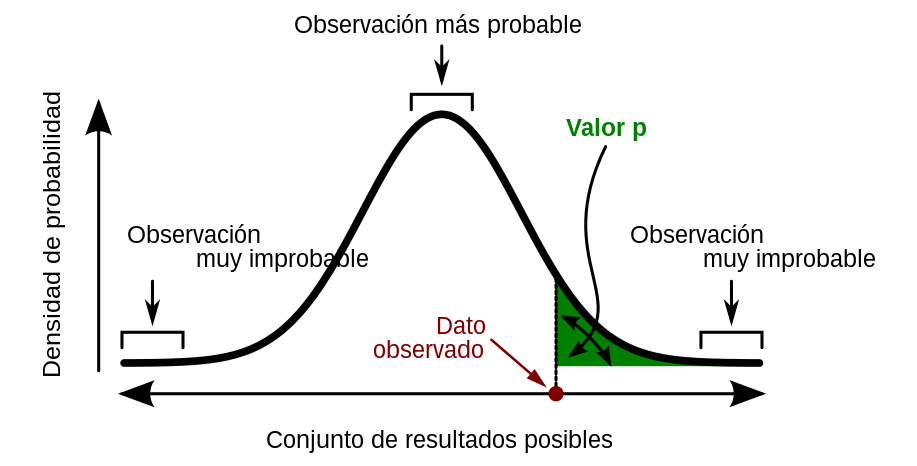
\includegraphics[width=0.7\linewidth]{img/Valor_p} 

}

\caption{Estadístico de prueba para un prueba altenativa con signo $>$}\label{fig:graficovalorp}
\end{figure}

La tabla \ref{tab:regiones}, da cuenta de la relación que existe entre las pruebas de hipótesis y la ubicación del valor-p en el gráfico presentado.

\begin{table}[H]

\caption{\label{tab:regiones}Hipótesis alternativa, valor-p y estadístico de prueba}
\centering
\begin{tabular}[t]{>{\centering\arraybackslash}p{4cm}>{\centering\arraybackslash}p{4cm}>{\centering\arraybackslash}p{5cm}}
\toprule
Signo de comparación en $H_1$ & Referencia & Ubicación del estadístico de prueba y valor-p\\
\midrule
$>$ & Unilateral derecha & A la derecha del gráfico\\
$<$ & Unilateral izquierda & A la izquierda del gráfico\\
$\neq$ & Bilateral & A ambos lados del gráfico\\
\bottomrule
\end{tabular}
\end{table}

La regla de rechazo usando el valor-p es

\[\text{Rechazar } H_0 \text{ si el valor-p } \leq \alpha\]

En la figura \ref{fig:regiones3}, se puede observar los tres casos posibles para las distintas hipótesis alternativas, en las cuales se ejemplifica un valor-p en cada uno de los casos. De izquierda a derecha, las hipótesis alternativas correspondientes son unilateral izquierda, unilateral derecha, y bilateral. La decisión de si en cada uno de los casos se rechaza o no la hipótesis nula, depende del valor elegido para la significancia.

\begin{figure}

{\centering 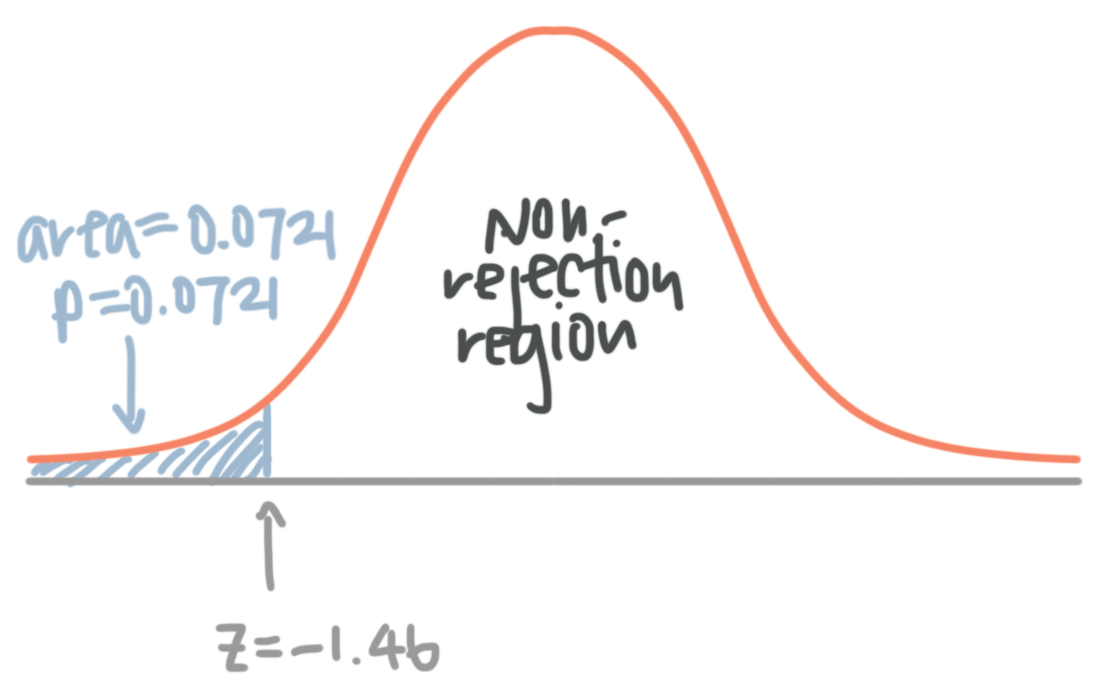
\includegraphics[width=0.3\linewidth]{img/R1} 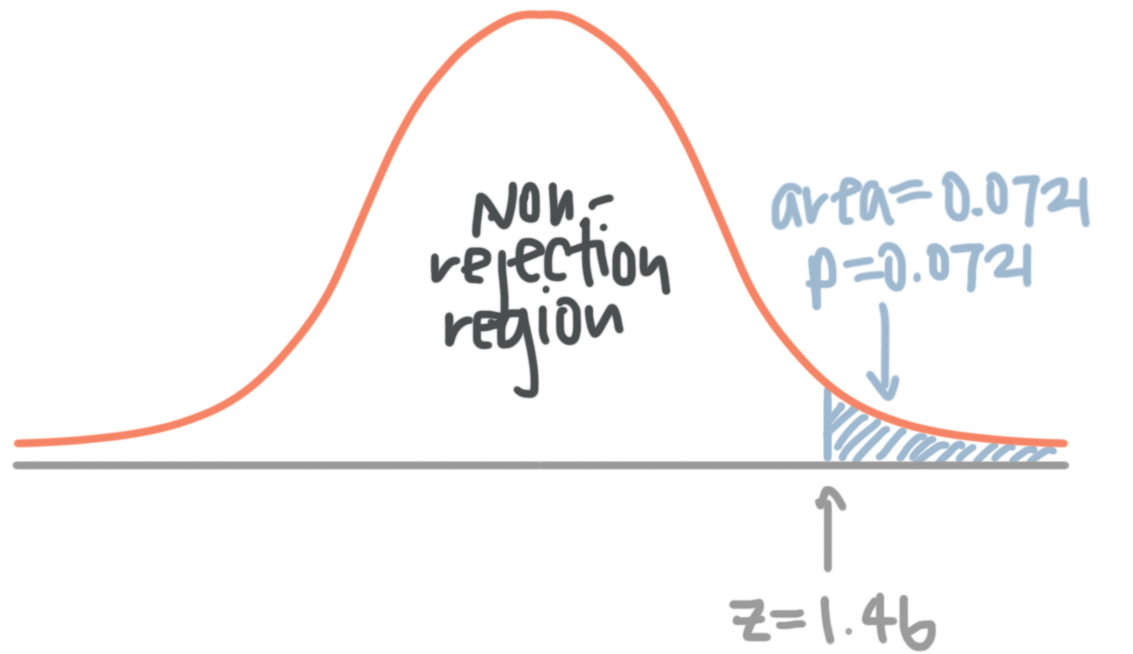
\includegraphics[width=0.3\linewidth]{img/R2} 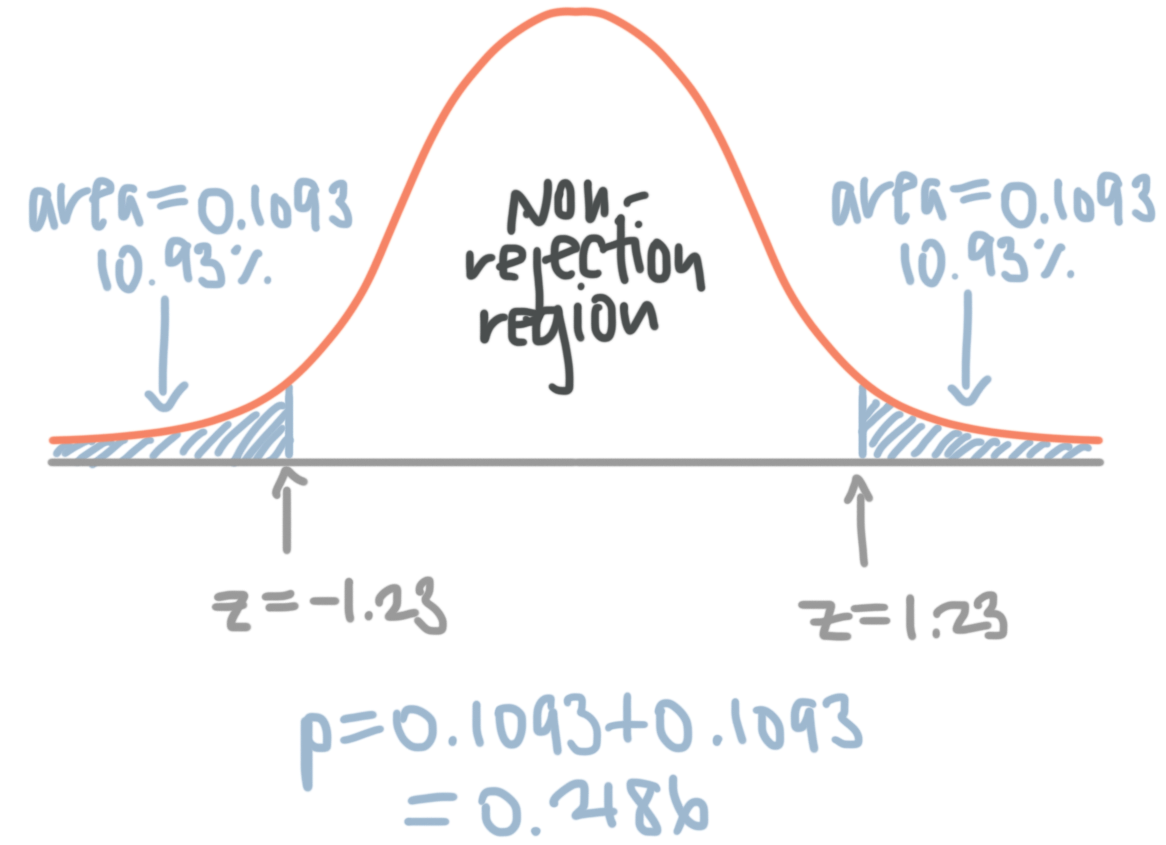
\includegraphics[width=0.3\linewidth]{img/R3} 

}

\caption{Estadísticos de prueba}\label{fig:regiones3}
\end{figure}

\begin{enumerate}
\def\labelenumi{\arabic{enumi}.}
\setcounter{enumi}{1}
\tightlist
\item
  \textbf{Método del valor crítico}
\end{enumerate}

Este método consiste en comparar el estadístico de prueba con un número fijo llamado \textbf{valor crítico}. El valor crítico es un punto de referencia para determinar si el valor del estadístico de prueba es lo suficientemente pequeño para rechazar la hipótesis nula. El valor
crítico corresponde a una porción del área bajo la curva, llamada \(\alpha\) (el cual es definido por el investigador), y está ubicada en el mismo sector que el valor-p.~

El intervalo de números generado a partir del valor crítico es lo denominado \textbf{región de rechazo}. En la figura \ref{fig:regiones2}, se observa que un hipótesis es rechazada cuando el valor-p es menor a \(\alpha\), lo cual, es equivalente a decir, que estadístico de prueba es mayor (o menor) al valor crítico, a esto se le denomina ``caer en la región de rechazo''.

\begin{figure}

{\centering 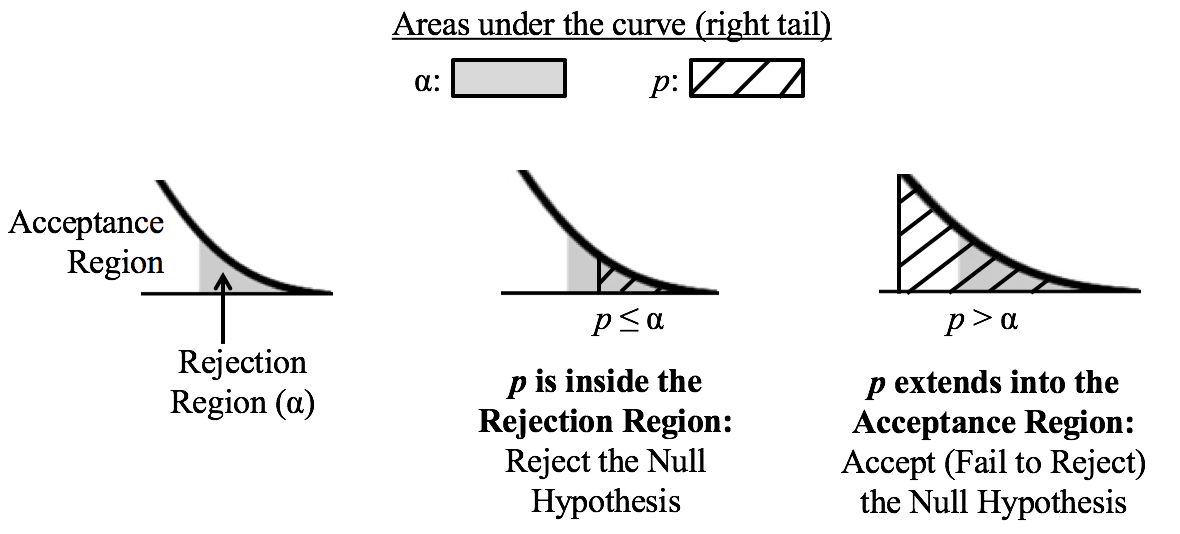
\includegraphics[width=0.8\linewidth]{img/RR} 

}

\caption{Valor-p, el área bajo la curva}\label{fig:regiones2}
\end{figure}

Los lineamiento de como construir un estadístico de prueba y un valor-p se darán a conocer a partir de la sección \ref{pruebas}.

\hypertarget{intervalos-de-confianza}{%
\subsection{Intervalos de confianza}\label{intervalos-de-confianza}}

Existe un relación directa entre las pruebas de hipótesis y los intervalos de confianza, ya que estos pueden ser utilizados para rechazar o no \(H_0\). La tabla \ref{tab:ICpruebas}, da cuenta de del tipo de intervalo de confianza que se debe elaborar para cada tipo de prueba de hipótesis.

\begin{table}[H]

\caption{\label{tab:ICpruebas}Hipótesis alternativa e Intervalo de confianza}
\centering
\begin{tabular}[t]{cc}
\toprule
Signo de comparación en $H_1$ & Tipo de intervalo de confianza\\
\midrule
$>$ & $(a,\infty )$\\
$<$ & $(-\infty ,b)$\\
$\neq$ & $(a,b)$\\
\bottomrule
\end{tabular}
\end{table}

A lo largo de las distintas pruebas, se abordarán los distintos métodos de prueba, incluyendo el uso de intervalos de confianza.

\hypertarget{pruebas}{%
\section{Pruebas de hipótesis para la media}\label{pruebas}}

Esta sección se centra en el planteamiento y prueba de hipótesis relacionadas a la parámetro de media. Para cada uno de estos casos, se detalla el procedimiento en R y los distintos métodos de prueba para la decisión de rechazo de \(H_0\). En particular, las pruebas para este parámetro requieren asumir la suposición de distribución normal de los datos.

\hypertarget{pruebas-de-hipuxf3tesis-para-la-media-de-una-distribuciuxf3n-normal-con-varianza-poblacional-conocida}{%
\subsection*{Pruebas de hipótesis para la media de una distribución normal con varianza poblacional conocida}\label{pruebas-de-hipuxf3tesis-para-la-media-de-una-distribuciuxf3n-normal-con-varianza-poblacional-conocida}}

Aun cuando la suposición de que el valor de \(\sigma^2\) es conocido, rara vez se cumple en la práctica. Este caso proporciona un buen punto de partida debido a la facilidad con que los procedimientos generales y sus propiedades pueden ser desarrollados. La hipótesis nula en los tres casos propondrá que \(\mu\) tiene un valor numérico particular, el valor nulo, el cual será denotado por \(\mu_0\).

El estadístico de prueba y los valores críticos de comparación están dados en la tabla \ref{tab:unamedia1}.

\begin{table}[H]

\caption{\label{tab:unamedia1}Criterios de rechazo para la prueba de una media con varianza poblacional conocida}
\centering
\begin{tabular}[t]{ll}
\toprule
\em{\textbf{Hipótesis nula}} & \em{\textbf{Estadístico}}\\
$H_0: \mu = \mu_0$ & $Z_0 = \displaystyle\frac{\bar{x}-\mu_0}{\sigma/\sqrt{n}}$\\
\em{\textbf{Hipótesis alternativa}} & \em{\textbf{Criterio de rechazo}}\\
$H_1: \mu \neq \mu_0$ & $|Z_0| \geq Z_{1-\alpha/2}$\\
$H_1: \mu \gt \mu_0$ & $Z_0 \geq Z_{1-\alpha}$\\
\addlinespace
$H_1: \mu \lt \mu_0$ & $Z_0 \leq Z_{\alpha}$\\
\bottomrule
\end{tabular}
\end{table}

\begin{example}
El índice Rockwell de dureza para acero se determina al presionar una punta de diamante en el acero y medir la profundidad de la penetración, el cual tiene un varianza de medición de 6. Para 50 especímenes de una aleación de acero, el índice Rockwell de dureza promedió 62. El fabricante dice que esta aleación tiene un índice de dureza promedio menor a 64. Asumiendo que el índice de dureza sigue una distribución normal, ¿hay suficiente evidencia para refutar lo dicho por el fabricante con un nivel de significancia de 1\%?

Al plantear la prueba de hipótesis se debe tener en cuenta que la hipótesis del investigador ha de estar reflejada en \(H_1\), tal como se muestra a continuación.

\begin{equation}
\notag
H_0: \mu = 64\\
H_1: \mu < 64
\end{equation}

Luego, se desarrolla la expresión del estadístico de prueba, para conocer su valor numérico.

\begin{equation}
\notag
Z_0 = \frac{\bar{x} - \mu_0}{\sigma/\sqrt{n}} = \displaystyle\frac{62 - 64}{\sqrt{6}/\sqrt{50}} = -5.774
\end{equation}

Ocupando el método del valor crítico, escribimos el criterios de rechazo correspondiente. Sin embargo, aún está la tarea de determinar el valor crítico.

\begin{equation}
\notag
\begin{split}
Z_0 &\leq Z_{\alpha}\\
-5.774 &\leq Z_{0.01}\\
\end{split}
\end{equation}

Para determinar el valor de \(Z_{0.01}\) (tal como menciona en los cursos de Estadística I y Estadística descriptiva), el comando a ocupar

\begin{Shaded}
\begin{Highlighting}[]
\FunctionTok{qnorm}\NormalTok{(}\AttributeTok{p =} \FloatTok{0.01}\NormalTok{)}
\end{Highlighting}
\end{Shaded}

\begin{verbatim}
## [1] -2.326348
\end{verbatim}

Es claro que \(-5.774\) es menor a \(-2.32\), es decir, que al cumplirse la condición de rechazo, esto implica que se rechaza \(H_0\). Por lo tanto, existe suficiente evidencia estadística para rechazar la hipótesis nula, es decir, se apoya la postura del fabricante respecto a un indice de dureza promedio menor a 64, con una significancia del 1\% (o confianza del 99\%).

En caso de que deseemos utilizar el método del valor-p, es necesario apoyarnos en R para realizar el calculo de este. El comando necesario para calcular el valor depende la prueba que estemos llevando a cabo, por lo que en el siguiente \href{https://github.com/Dfranzani/Estadistica_II_UDP/blob/main/resumenes/Rechazo.pdf}{documento} podrán encontrar un resumen para las distintas pruebas.

\begin{Shaded}
\begin{Highlighting}[]
\FunctionTok{pnorm}\NormalTok{(}\SpecialCharTok{{-}}\FloatTok{5.774}\NormalTok{)}
\end{Highlighting}
\end{Shaded}

\begin{verbatim}
## [1] 3.870572e-09
\end{verbatim}

El valor-p obtenido es evidentemente menor a la significancia (0.01), obteniéndose la misma conclusión antes expuesta.

Respecto al intervalo de confianza, es posible determinarlo dada la siguiente expresión.

\begin{equation}
\left(-\infty, \bar{x} + Z_{1-\alpha}\frac{\sigma}{\sqrt{n}}\right)
\end{equation}

Reemplazando los valores dados en el enunciado se tiene

\begin{equation}
\notag
\left(-\infty, 62 + Z_{0.99}\frac{6}{\sqrt{50}}\right) = (-\infty, 62.71)
\end{equation}

Al observar el intervalo de confianza, se debe observar si el valor de \(\mu_0\) está dentro o fuera de este. En este caso, \(\mu_0 = 64\) no se encuentra dentro del intervalo. Por lo tanto, se rechaza la hipótesis nula, obteniéndose la misma conclusión antes obtenida.

Al igual que el valor-p, la forma en la que se debe usar el intervalo de confianza varía dependiendo del tipo de prueba de hipótesis que se realiza, por lo que en el siguiente \href{https://github.com/Dfranzani/Estadistica_II_UDP/blob/main/resumenes/Resumen\%20de\%20intervalos\%20de\%20Hip\%C3\%B3tesis\%20e\%20IC.pdf}{documento} podrán encontrar un resumen para las distintas pruebas, dicho documento incluye los distintos comando en R para obtener los resultados de una prueba de hipótesis de manera automática.
\end{example}

Para este tipo de pruebas, no hay comandos en R que permitan hacer el trabajo de manera automática. Esto es debido a lo expuesto en un principio: \textbf{difícilmente se conoce la varianza poblacional en la práctica}.

\begin{exercise}

Sea el estadístico de prueba \(Z\) con una distribución normal estándar cuando \(H_0\) es verdadera. Dé el nivel de significación en cada una de las siguientes situaciones:

\begin{enumerate}
\def\labelenumi{\alph{enumi}.}
\tightlist
\item
  \(H_1: \mu > \mu_0\), región de rechazo \(z\geq 1.88\).
\item
  \(H_1: \mu < \mu_0\), región de rechazo \(z\leq -2.75\).
\item
  \(H_1: \mu \neq \mu_0\), región de rechazo \(z\geq 2.88\) o \(z\leq -2.88\).
\end{enumerate}

\end{exercise}

\begin{exercise}
Un fabricante de cajas de cartón afirma que sus cajas tienen un peso promedio de 5 kg. Para verificar esta afirmación, un cliente selecciona al azar 25 cajas y encuentra que el peso promedio es de 4.8 kg con una desviación estándar conocida de 0.5 kg. ¿Hay suficiente evidencia para rechazar la afirmación del fabricante al nivel de significancia del 5\%?
\end{exercise}

\begin{exercise}
Un entrenador de baloncesto cree que sus jugadores pueden hacer tiros libres con una precisión de al menos el 80\%. Para probar su hipótesis, el entrenador toma una muestra aleatoria de 30 tiros libres y encuentra que la proporción de tiros exitosos es del 75\%. Si la desviación estándar conocida de la proporción de tiros exitosos es del 5\%, ¿hay suficiente evidencia para rechazar la hipótesis del entrenador al nivel de significancia del 1\%?
\end{exercise}

\begin{exercise}
Un cirujano afirma que sus pacientes se recuperan en un promedio de 5 días después de una cirugía. Para probar su afirmación, el cirujano toma una muestra aleatoria de 20 pacientes y encuentra que la duración promedio de recuperación es de 6 días, con una desviación estándar conocida de 1.5 días. ¿Hay suficiente evidencia para rechazar la afirmación del cirujano al nivel de significancia del 10\%?
\end{exercise}

\begin{exercise}
Se cree que la cantidad promedio de cafeína en una taza de café es de 100 mg. Para probar esta hipótesis, se toma una muestra aleatoria de 50 tazas de café y se encuentra que la cantidad promedio de cafeína es de 105 mg, con una desviación estándar conocida de 15 mg. ¿Hay suficiente evidencia para rechazar la hipótesis nula al nivel de significancia del 5\%?
\end{exercise}

\begin{exercise}
Se desea evaluar si la altura promedio de una población de girasoles es de 150 cm. Para ello, se selecciona una muestra aleatoria de 30 girasoles y se encuentra que la altura promedio es de 155 cm, con una desviación estándar conocida de 5 cm. ¿Hay suficiente evidencia para rechazar la hipótesis nula al nivel de significancia del 1\%?
\end{exercise}

\hypertarget{pruebas-de-hipuxf3tesis-para-la-media-de-una-distribuciuxf3n-normal-con-varianza-poblacional-desconocida}{%
\subsection*{Pruebas de hipótesis para la media de una distribución normal con varianza poblacional desconocida}\label{pruebas-de-hipuxf3tesis-para-la-media-de-una-distribuciuxf3n-normal-con-varianza-poblacional-desconocida}}

De igual manera los expuesto en el primer caso, los pasos a seguir para probar una hipótesis son los mismo, y se mantendra así para cualquier caso.

\begin{enumerate}
\def\labelenumi{\arabic{enumi}.}
\tightlist
\item
  Plantear las hipótesis nula y alternativa
\item
  Identificar o establecer el nivel de significancia.
\item
  Identificar los datos muestrales y poblacionales con los que se cuenta.
\item
  Utilizar alguna de las reglas de decisión (Estadístico de prueba, valor-p o intervalo de confianza).
\item
  Concluir
\end{enumerate}

En la situación de una prueba de hipótesis de la media, en la cual lo datos distribuyen normal y la varianza poblacional es desconocida, los criterios de rechazo son similares a los vistos anteriormente, sin embargo, cambia la distribución del estadístico de prueba, tal como se muestra en la tabla xxx.

\begin{table}[H]

\caption{\label{tab:unamedia2}Criterios de rechazo para la prueba de una media con varianza poblacional conocida}
\centering
\begin{tabular}[t]{ll}
\toprule
\em{\textbf{Hipótesis nula}} & \em{\textbf{Estadístico}}\\
$H_0: \mu = \mu_0$ & $t_0 = \displaystyle\frac{\bar{x}-\mu_0}{S/\sqrt{n}}$\\
\em{\textbf{Hipótesis alternativa}} & \em{\textbf{Criterio de rechazo}}\\
$H_1: \mu \neq \mu_0$ & $|t_0| \geq t_{1-\alpha/2, n-1}$\\
$H_1: \mu \gt \mu_0$ & $t_0 \geq t_{1-\alpha,n-1}$\\
\addlinespace
$H_1: \mu \lt \mu_0$ & $t_0 \leq t_{\alpha,n-1}$\\
\bottomrule
\end{tabular}
\end{table}

donde \(n\) corresponde al tamaño de la muestra.

\begin{example}
\protect\hypertarget{exm:imacec}{}\label{exm:imacec}\textbf{(Portafolio 2022, segundo semestre, pregunta 2)} La base de datos \href{https://raw.githubusercontent.com/Dfranzani/Bases-de-datos-para-cursos/main/2022-2/Estad\%C3\%ADstica\%201/imacec.csv}{\emph{imacec.csv}}, contiene los datos del Imacec del área de producción de bienes en los sectores de Minería e Industria, desde enero de 2018 hasta junio de 2022. Establezca si hay suficiente evidencia estadística, para afirmar que, el valor promedio del Imacec de cada sector por separado, es mayor al promedio general de todos los sectores (denote el promedio general por \(\mu_0\)). Establezca las hipótesis respectivas, estadísticos y criterios de rechazo, utilizando una significancia del 10\%. Asume que las variables distribuyen normal y tienen varianza poblacional desconocida.

En este caso al contar con una base de datos (y para este tipo de prueba), podemos hacer uso directamente de R para obtener el estadístico de prueba, valor-p e intervalo de confianza asociado.

\begin{Shaded}
\begin{Highlighting}[]
\CommentTok{\# Carga de la base de datos}
\NormalTok{df }\OtherTok{=} \FunctionTok{read.csv}\NormalTok{(}\StringTok{"https://raw.githubusercontent.com/Dfranzani/Bases{-}de{-}datos{-}para{-}cursos/main/2022{-}2/Estad\%C3\%ADstica\%201/imacec.csv"}\NormalTok{)}
\end{Highlighting}
\end{Shaded}

En primer lugar, obtenemos el valor de \(mu_0\) para poder plantear la prueba de hipótesis

\begin{Shaded}
\begin{Highlighting}[]
\CommentTok{\# Promedio de todos los sectores}
\NormalTok{promedio\_general }\OtherTok{=} \FunctionTok{mean}\NormalTok{(}\FunctionTok{c}\NormalTok{(df}\SpecialCharTok{$}\NormalTok{Mineria, }\CommentTok{\# Valores del Imacec de Minería}
\NormalTok{                          df}\SpecialCharTok{$}\NormalTok{Industria)) }\CommentTok{\# Valores del Imacec de Industria}
\NormalTok{promedio\_general }\CommentTok{\# Mu\_0}
\end{Highlighting}
\end{Shaded}

\begin{verbatim}
## [1] 98.54167
\end{verbatim}

Iniciamos con la prueba de hipótesis para el sector de minería.

\begin{equation}
    \notag
    \begin{split}
        H_0: \mu_{\text{Imacec-Mineria}} = 98.54167\\
        H_1: \mu_{\text{Imacec-Mineria}} > 98.54167
    \end{split}
\end{equation}

Luego, haciendo uso de R obtenemos los elementos necesario para rechazar o no \(H_0\).

\begin{Shaded}
\begin{Highlighting}[]
\CommentTok{\# Minería}
\FunctionTok{t.test}\NormalTok{( }\CommentTok{\# Prueba de hipótesis para el estadístico con distribución t{-}student}
  \AttributeTok{x =}\NormalTok{ df}\SpecialCharTok{$}\NormalTok{Mineria, }\CommentTok{\# Valores del Imacec de Minería}
  \AttributeTok{alternative =} \StringTok{"greater"}\NormalTok{, }\CommentTok{\# Signo de desigualdad de la hipótesis alternativa}
  \AttributeTok{mu =} \FloatTok{98.54167}\NormalTok{, }\CommentTok{\# Valor del Mu\_0}
  \AttributeTok{conf.level =} \FloatTok{0.9} \CommentTok{\# Confianza = 1 {-} alfa}
\NormalTok{  )}
\end{Highlighting}
\end{Shaded}

\begin{verbatim}
## 
##  One Sample t-test
## 
## data:  df$Mineria
## t = -1.2773, df = 53, p-value = 0.8965
## alternative hypothesis: true mean is greater than 98.54167
## 90 percent confidence interval:
##  96.21024      Inf
## sample estimates:
## mean of x 
##  97.38519
\end{verbatim}

El estadístico reportado es \(t = -1.27373\) con un valor-p de 0.8965, el cual, al ser mayor a la significancia de 0.05, implica que no existe suficiente evidencia estadística para rechazar \(H_0\), por lo que se asume que, el valor promedio del Imacec del sector de Minería no es mayor al promedio de general de ambos sectores.

Utilizando el intervalo de confianza \((96.21, \infty)\), se observa que el valor de \(\mu_0 = 98.54\) se encuentra dentro del intervalo, por ende, no existe suficiente evidencia estadística para rechazar \(H_0\), obteniéndose la misma conclusión que al usar el valor-p.

La prueba de hipótesis para el sector de industria es la siguiente.

\begin{equation}
    \notag
    \begin{split}
        H_0: \mu_{\text{Imacec-Industria}} = 98.54167\\
        H_1: \mu_{\text{Imacec-Industria}} > 98.54167
    \end{split}
\end{equation}

\begin{Shaded}
\begin{Highlighting}[]
\CommentTok{\# Industria}
\FunctionTok{t.test}\NormalTok{( }\CommentTok{\# Prueba de hipótesis para el estadístico con distribución t{-}student}
  \AttributeTok{x =}\NormalTok{ df}\SpecialCharTok{$}\NormalTok{Industria, }\CommentTok{\# Valores del Imacec de Industria}
  \AttributeTok{alternative =} \StringTok{"greater"}\NormalTok{, }\CommentTok{\# Signo de desigualdad de la hipótesis alternativa}
  \AttributeTok{mu =} \FloatTok{98.54167}\NormalTok{, }\CommentTok{\# Valor del Mu\_0}
  \AttributeTok{conf.level =} \FloatTok{0.9} \CommentTok{\# Confianza = 1 {-} alfa}
\NormalTok{  )}
\end{Highlighting}
\end{Shaded}

\begin{verbatim}
## 
##  One Sample t-test
## 
## data:  df$Industria
## t = 1.3678, df = 53, p-value = 0.08857
## alternative hypothesis: true mean is greater than 98.54167
## 90 percent confidence interval:
##  98.60095      Inf
## sample estimates:
## mean of x 
##  99.69815
\end{verbatim}

El estadístico reportado es \(t = 1.3678\) con un valor-p de 0.08857, el cual, al ser mayor a la significancia de 0.1, implica que existe suficiente evidencia estadística para rechazar \(H_0\), por lo que se asume que, el valor promedio del Imacec del sector de Industria es mayor al promedio de general de ambos sectores.

Utilizando el intervalo de confianza \((98.6, \infty)\), se observa que el valor de \(\mu_0 = 98.54\) no se encuentra dentro del intervalo, por ende, no existe suficiente evidencia estadística para rechazar \(H_0\), obteniéndose la misma conclusión que al usar el valor-p.
\end{example}

\begin{exercise}
Utilizando la base del ejemplo \ref{exm:imacec}. Establezca si hay suficiente evidencia estadística para afirmar que, el valor promedio del Imacec de cada sector durante el año 2022, es mayor al promedio general de todos los sectores en el mismo año (denote el promedio general por \(\mu_{0}\)). Establezca las hipótesis respectivas, estadísticos y criterios de rechazo, utilice una significancia del 7\%. Asuma que las variables distribuyen normal y tienen varianza poblacional desconocida. Concluya.
\end{exercise}

\begin{exercise}
\protect\hypertarget{exr:metano}{}\label{exr:metano}El control de emisión de residuos ha sido un tema que ha cobrado gran importancia en los últimos 20 años debido a los efectos del calentamiento global. Uno de los tantos residuos que contamina el aire es el Metano (CH4). Para estudiar este fenómeno haremos uso de la base \href{https://raw.githubusercontent.com/Dfranzani/Bases-de-datos-para-cursos/main/2022-2/Estad\%C3\%ADstica\%202/metano.csv}{\emph{metano.csv}}, la cual contiene los siguientes datos:

\begin{itemize}
\tightlist
\item
  Año: año en el que se realiza la medición de emisión de CH4.
\item
  Mes: mes del año en el que se realiza la medición de emisión de CH4.
\item
  CH4: concentración de CH4 (partes por miles de millones) en un muestra de aire.
\end{itemize}

Establezca si hay suficiente evidencia estadística para afirmar los siguiente:

\begin{enumerate}
\def\labelenumi{\arabic{enumi}.}
\tightlist
\item
  La concentración promedio de metano es distinta a 1700 partes por millón.
\item
  La concentración promedio de metano del año 2021 es superior a 1780 partes por millón.
\item
  La concentración promedio de metano del periodo en el periodo de años 2019 - 2022 (inclusive) es inferior a 1750 partes por millón.
\end{enumerate}

Establezca las hipótesis respectivas, estadísticos y criterios de rechazo, utilice una significancia del 7\%. Asuma que las variables distribuyen normal y tienen varianza poblacional desconocida. Concluya.
\end{exercise}

\begin{exercise}
\protect\hypertarget{exr:consumidor}{}\label{exr:consumidor}La base de datos \href{https://raw.githubusercontent.com/Dfranzani/Bases-de-datos-para-cursos/main/2022-2/Estad\%C3\%ADstica\%202/consumidor.csv}{\emph{consumidor.csv}} contiene registros del Índice de Confianza del Consumidor (ICC). Este indicador de confianza del consumidor proporciona una indicación de la evolución futura del consumo y el ahorro de los hogares. Un indicador por encima de 100 señala un aumento en la confianza de los consumidores hacia la situación económica futura, como consecuencia de la cual son menos propensos a ahorrar y más inclinados a gastar dinero en compras importantes en los próximos 12 meses. Los valores por debajo de 100 indican una actitud pesimista hacia la evolución futura de la economía, lo que posiblemente resulte en una tendencia a ahorrar más y consumir menos.

Las variables que contiene la base de datos son las siguientes:

\begin{itemize}
\tightlist
\item
  Locacion: lugar en donde se mide el ICC (FRA = Francia, POL = Polonia, OECD = OCDE, ESP = España, BEL = Bélgica, ITA = Italia, DEU = Alemania).
\item
  Mes: corresponde al mes en el que se realiza la medición del índice.
\item
  Ano: corresponde al año en el que se realiza la medición del índice.
\item
  ICC: valor del índice de confianza del consumidor.
\end{itemize}

Establezca si hay suficiente evidencia estadística para afirmar los siguiente:

\begin{enumerate}
\def\labelenumi{\arabic{enumi}.}
\tightlist
\item
  El promedio del ICC es distinto a 100 puntos.
\item
  El promedio del ICC en Francia es menor a 105 puntos.
\item
  El promedio del ICC en Alemania es mayor a 107 puntos.
\end{enumerate}

Establezca las hipótesis respectivas, estadísticos y criterios de rechazo, utilice una significancia del 12\%. Asuma que las variables distribuyen normal y tienen varianza poblacional desconocida. Concluya.
\end{exercise}

\hypertarget{pruebas-de-hipuxf3tesis-para-la-diferencia-de-medias}{%
\section{Pruebas de hipótesis para la diferencia de medias}\label{pruebas-de-hipuxf3tesis-para-la-diferencia-de-medias}}

\hypertarget{prueba-de-hipuxf3tesis-para-la-diferencia-de-medias-de-dos-distribuciones-normales-con-varianzas-poblacionales-conocidas}{%
\subsection*{Prueba de hipótesis para la diferencia de medias de dos distribuciones normales con varianzas poblacionales conocidas}\label{prueba-de-hipuxf3tesis-para-la-diferencia-de-medias-de-dos-distribuciones-normales-con-varianzas-poblacionales-conocidas}}

\hypertarget{prueba-de-hipuxf3tesis-para-la-diferencia-de-medias-de-dos-distribuciones-normales-con-varianzas-poblacionales-desconocidas-e-iguales}{%
\subsection*{Prueba de hipótesis para la diferencia de medias de dos distribuciones normales con varianzas poblacionales desconocidas e iguales}\label{prueba-de-hipuxf3tesis-para-la-diferencia-de-medias-de-dos-distribuciones-normales-con-varianzas-poblacionales-desconocidas-e-iguales}}

\hypertarget{prueba-de-hipuxf3tesis-para-la-diferencia-de-medias-de-dos-distribuciones-normales-con-varianzas-poblacionales-desconocidas-y-distintas}{%
\subsection*{Prueba de hipótesis para la diferencia de medias de dos distribuciones normales con varianzas poblacionales desconocidas y distintas}\label{prueba-de-hipuxf3tesis-para-la-diferencia-de-medias-de-dos-distribuciones-normales-con-varianzas-poblacionales-desconocidas-y-distintas}}

\hypertarget{prueba-de-hipuxf3tesis-para-comparaciuxf3n-de-varianzas}{%
\section{Prueba de hipótesis para comparación de varianzas}\label{prueba-de-hipuxf3tesis-para-comparaciuxf3n-de-varianzas}}

\hypertarget{prueba-de-hipuxf3tesis-para-la-diferencia-de-proporciones}{%
\section{Prueba de hipótesis para la diferencia de proporciones}\label{prueba-de-hipuxf3tesis-para-la-diferencia-de-proporciones}}

\hypertarget{regresiuxf3n-lineal}{%
\chapter{Regresión Lineal}\label{regresiuxf3n-lineal}}

\hypertarget{anuxe1lisis-descriptivo-de-datos}{%
\section{Análisis descriptivo de datos}\label{anuxe1lisis-descriptivo-de-datos}}

\hypertarget{gruxe1ficos}{%
\subsection{Gráficos}\label{gruxe1ficos}}

\hypertarget{tablas}{%
\subsection{Tablas}\label{tablas}}

\hypertarget{covarianza}{%
\section{Covarianza}\label{covarianza}}

\hypertarget{correlaciuxf3n}{%
\section{Correlación}\label{correlaciuxf3n}}

\hypertarget{regresiuxf3n-lineal-simple}{%
\section{Regresión lineal simple}\label{regresiuxf3n-lineal-simple}}

\hypertarget{suma-cuadruxe1tica-de-errores}{%
\subsection{Suma cuadrática de errores}\label{suma-cuadruxe1tica-de-errores}}

\hypertarget{estimadores-de-muxednimos-cuadrados}{%
\subsection{Estimadores de mínimos cuadrados}\label{estimadores-de-muxednimos-cuadrados}}

\hypertarget{pruebas-de-hipuxf3tesis-1}{%
\subsection{Pruebas de hipótesis}\label{pruebas-de-hipuxf3tesis-1}}

\hypertarget{supuestos}{%
\subsection{Supuestos}\label{supuestos}}

\hypertarget{linealidad}{%
\subsubsection*{Linealidad}\label{linealidad}}

\hypertarget{normalidad}{%
\subsubsection*{Normalidad}\label{normalidad}}

\hypertarget{homocedasticidad}{%
\subsubsection*{Homocedasticidad}\label{homocedasticidad}}

\hypertarget{independencia}{%
\subsubsection*{Independencia}\label{independencia}}

\hypertarget{error-estuxe1ndar-residual}{%
\subsection{Error estándar residual}\label{error-estuxe1ndar-residual}}

\hypertarget{coeficiente-de-determinaciuxf3n}{%
\subsection{Coeficiente de determinación}\label{coeficiente-de-determinaciuxf3n}}

\hypertarget{regresiuxf3n-lineal-muxfaltiple}{%
\section{Regresión lineal múltiple}\label{regresiuxf3n-lineal-muxfaltiple}}

\hypertarget{suma-cuadruxe1tica-de-errores-1}{%
\subsection{Suma cuadrática de errores}\label{suma-cuadruxe1tica-de-errores-1}}

\hypertarget{suma-cuadruxe1tica-total}{%
\subsection{Suma cuadrática total}\label{suma-cuadruxe1tica-total}}

\hypertarget{estimadores-de-muxednimos-cuadrados-1}{%
\subsection{Estimadores de mínimos cuadrados}\label{estimadores-de-muxednimos-cuadrados-1}}

\hypertarget{pruebas-de-hipuxf3tesis-2}{%
\subsection{Pruebas de hipótesis}\label{pruebas-de-hipuxf3tesis-2}}

\hypertarget{supuestos-1}{%
\subsection{Supuestos}\label{supuestos-1}}

\hypertarget{linealidad-1}{%
\subsubsection*{Linealidad}\label{linealidad-1}}

\hypertarget{normalidad-1}{%
\subsubsection*{Normalidad}\label{normalidad-1}}

\hypertarget{homocedasticidad-1}{%
\subsubsection*{Homocedasticidad}\label{homocedasticidad-1}}

\hypertarget{independencia-1}{%
\subsubsection*{Independencia}\label{independencia-1}}

\hypertarget{error-estuxe1ndar-residual-1}{%
\subsection{Error estándar residual}\label{error-estuxe1ndar-residual-1}}

\hypertarget{coeficiente-de-determinaciuxf3n-ajustado}{%
\subsection{Coeficiente de determinación ajustado}\label{coeficiente-de-determinaciuxf3n-ajustado}}

\hypertarget{selecciuxf3n-de-variables}{%
\section{Selección de variables}\label{selecciuxf3n-de-variables}}

\hypertarget{forward}{%
\subsection{Forward}\label{forward}}

\hypertarget{backward}{%
\subsection{Backward}\label{backward}}

\hypertarget{anova-y-pruebas-no-paramuxe9tricas}{%
\chapter{ANOVA y pruebas no paramétricas}\label{anova-y-pruebas-no-paramuxe9tricas}}

\hypertarget{anova-de-un-factor}{%
\section{ANOVA de un factor}\label{anova-de-un-factor}}

\hypertarget{varianzas}{%
\subsection{Varianzas}\label{varianzas}}

\hypertarget{condiciones}{%
\subsection{Condiciones}\label{condiciones}}

\hypertarget{tamauxf1o-del-efecto}{%
\subsection{Tamaño del efecto}\label{tamauxf1o-del-efecto}}

\hypertarget{anova-de-dos-factores}{%
\section{ANOVA de dos factores}\label{anova-de-dos-factores}}

\hypertarget{varianzas-1}{%
\subsection{Varianzas}\label{varianzas-1}}

\hypertarget{condiciones-1}{%
\subsection{Condiciones}\label{condiciones-1}}

\hypertarget{tamauxf1o-del-efecto-1}{%
\subsection{Tamaño del efecto}\label{tamauxf1o-del-efecto-1}}

\hypertarget{anuxe1lisis-de-homogeneidad-de-varianzas}{%
\section{Análisis de homogeneidad de varianzas}\label{anuxe1lisis-de-homogeneidad-de-varianzas}}

\hypertarget{prueba-de-levene-y-barlett}{%
\subsection{Prueba de Levene y Barlett}\label{prueba-de-levene-y-barlett}}

\hypertarget{pruebas-no-paramuxe9tricas}{%
\section{Pruebas no paramétricas}\label{pruebas-no-paramuxe9tricas}}

\hypertarget{pruebas-de-los-rangos-signados}{%
\subsection{Pruebas de los rangos signados}\label{pruebas-de-los-rangos-signados}}

\hypertarget{prueba-de-w-m-w}{%
\subsection{Prueba de W-M-W}\label{prueba-de-w-m-w}}

\hypertarget{prueba-de-kruskall---wallis}{%
\subsection{Prueba de Kruskall - Wallis}\label{prueba-de-kruskall---wallis}}

  \bibliography{refs.bib}

\end{document}
